\documentclass[UTF8]{ctexart}
\usepackage{amsmath}  %加载公式
\usepackage{graphicx}
\usepackage{setspace} %调整行间距
%\usepackage{CJKutf8}
\usepackage{indentfirst}        %首行缩进宏包
\usepackage{latexsym,bm}        % 处理数学公式中和黑斜体的宏包
\usepackage{amsmath,amssymb}    % AMSLaTeX宏包 用来排出更加漂亮的公式

\usepackage{cases}
\usepackage{pifont}
\usepackage{txfonts}
%%%%%%%%%%% CJK下设置中文字体 %%%%%%%%%%%%%
\newcommand{\song}{\CJKfamily{song}}   % 宋体 
\newcommand{\fs}{\CJKfamily{fs}}        % 仿宋体 (Windows自带simfs.ttf)
\newcommand{\kai}{\CJKfamily{kai}}      % 楷体   (Windows自带simkai.ttf)
\newcommand{\hei}{\CJKfamily{hei}}      % 黑体   (Windows自带simhei.ttf)
\newcommand{\li}{\CJKfamily{li}}        % 隶书   (Windows自带simli.ttf)
%%%%%%%%%%%  设置字体大小 %%%%%%%%%%%%%
\newcommand{\chuhao}{\fontsize{42pt}{\baselineskip}\selectfont}
\newcommand{\xiaochuhao}{\fontsize{36pt}{\baselineskip}\selectfont}
\newcommand{\yihao}{\fontsize{28pt}{\baselineskip}\selectfont}
\newcommand{\erhao}{\fontsize{21pt}{\baselineskip}\selectfont}
\newcommand{\xiaoerhao}{\fontsize{18pt}{\baselineskip}\selectfont}
\newcommand{\sanhao}{\fontsize{15.75pt}{\baselineskip}\selectfont}
\newcommand{\sihao}{\fontsize{14pt}{\baselineskip}\selectfont}
\newcommand{\xiaosihao}{\fontsize{12pt}{\baselineskip}\selectfont}
\newcommand{\wuhao}{\fontsize{10.5pt}{\baselineskip}\selectfont}
\newcommand{\xiaowuhao}{\fontsize{9pt}{\baselineskip}\selectfont}
\newcommand{\liuhao}{\fontsize{7.875pt}{\baselineskip}\selectfont}
\newcommand{\qihao}{\fontsize{5.25pt}{\baselineskip}\selectfont}

%%%% 设置 section 属性 %%%%
\makeatletter
\renewcommand\section{\@startsection{section}{1}{\z@}%
	{-1.5ex \@plus -.5ex \@minus -.2ex}%
	{1.5ex \@plus .1ex}%
	{\normalfont\sanhao\CJKfamily{song}}}
\makeatother

%%%% 设置 subsection 属性 %%%%
\makeatletter
\renewcommand\subsection{\@startsection{subsection}{1}{\z@}%
	{-1.25ex \@plus -.5ex \@minus -.2ex}%
	{.4ex \@plus .1ex}%
	{\normalfont\sihao\CJKfamily{song}}}
\makeatother

%%%% 设置 subsubsection 属性 %%%%
\makeatletter
\renewcommand\subsubsection{\@startsection{subsubsection}{1}{\z@}%
	{-1ex \@plus -.5ex \@minus -.2ex}%
	{.3ex \@plus .1ex}%
	{\normalfont\xiaosihao\CJKfamily{song}}}
\makeatother

%%%% 段落首行缩进两个字 %%%%
\makeatletter
\let\@afterindentfalse\@afterindenttrue
\@afterindenttrue
\makeatother
\setlength{\parindent}{2em}  %中文缩进两个汉字位


%%%% 下面的命令重定义页面边距,使其符合中文刊物习惯 %%%%
\addtolength{\topmargin}{-54pt}
\setlength{\oddsidemargin}{0.63cm}  % 3.17cm - 1 inch
\setlength{\evensidemargin}{\oddsidemargin}
\setlength{\textwidth}{14.66cm}
\setlength{\textheight}{24.00cm}    % 24.62

%%%% 下面的命令设置行间距与段落间距 %%%%
\linespread{1.2}
\setlength{\parskip}{1ex}
%\setlength{\parskip}{\baselineskip}


\begin{document}
	\thispagestyle{empty}
	\newtheorem{example}{例}             % 整体编号
	\newtheorem{algorithm}{算法}
	\newtheorem{theorem}{定理}[section]  % 按 section 编号
	\newtheorem{definition}{定义}
	\newtheorem{axiom}{公理}
	\newtheorem{property}{性质}
	\newtheorem{proposition}{命题}
	\newtheorem{lemma}{引理}
	\newtheorem{corollary}{推论}
	\newtheorem{remark}{注解}
	\newtheorem{condition}{条件}
	\newtheorem{conclusion}{结论}
	\newtheorem{assumption}{假设}
	
	%%%% 重定义 %%%%
	\renewcommand{\contentsname}{目录}  % 将Contents改为目录
	\renewcommand{\abstractname}{摘要}  % 将Abstract改为摘要
	\renewcommand{\refname}{参考文献}   % 将References改为参考文献
	\renewcommand{\indexname}{索引}
	\renewcommand{\figurename}{图}
	\renewcommand{\tablename}{表}
	\renewcommand{\appendixname}{附录}
	\renewcommand{\algorithm}{算法}
	\renewcommand{\baselinestretch}{1.2}



	\title{Automatically Labeled Data Generation for Large Scale Event Extraction\\大规模事件抽取的自动标记数据生成}
	
	\date{2020年}
	\pagestyle{plain}  %%%不要页眉,页脚包含一个居中的页码
	\thispagestyle{empty}  %%这一页不要页码
	\maketitle
	\tableofcontents
	
	\newpage
	  
	\begin{abstract}
	
	大多数事件抽取任务都依赖于人工标注数据,但是人工标注数据十分昂贵,事件类型少,每个事件类型数量也少,因此有监督的事件抽取很难利用到大规模事件抽取中。本文提出利用知识库(Freebase和FrameNet,Wikipedia)来自动标记数据。本文自动标记的数据包含人工标注的数据,可以从人工标注的数据中提升性能。
	
	\end{abstract}

	\newpage
	\setcounter{page}{1}  %%%这一页开始设置页码为1
	\section{简介}
	\textbf{ACE的缺点:}  %%%文字加粗
	\begin{enumerate}
		\item ACE数据集中,33个事件类型是在599个英文文档中人工标注的。
		\item ACE数据集中60\%的事件类型都是少于一百个样例,甚至有三个事件类型是少于10个样本的。
		\item 预定义的33个事件类型不能运用到大规模事件抽取中。
	\end{enumerate}
	图一是标记句子的示例。\\
	\begin{figure}[ht]
	\centering
	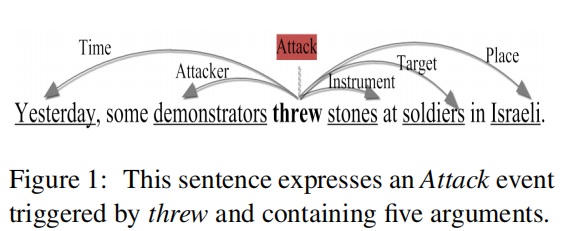
\includegraphics[width = .8\textwidth]{1.png} \\ %加载图片,缩放至页面的80%
	\caption{示例}
	\end{figure}

	\textbf{将远程监督(DS)运用到事件抽取的挑战:}
	\begin{itemize}
		\item 在知识库中,触发词并不是提前给出的。为了解决这个问题,文在运用远程监督之前,先发现触发词,再去自动标记事件元素。
		\item 根据远程监督在关系抽取内的应用,我们假设一个句子包含所有的事件元素,然而,对于特定事件,元素是分布在多个句子中。
	\end{itemize}
	
	为了解决上述问题,我们提出一个方法利用Freebase和FrameNet来为大规模事件抽取自动标记数据。
	首先,我们提出了一种利用Freebase对每种事件类型的参数进行优先级排序和选择关键参数或代表参数的方法(详见3.1节);其次,我们只使用关键参数来标记事件并找出触发词;第三,外部语言知识资源FrameNet,然后,我们提出了一种 Soft Distant Supervision(SDS)方法,它可以自动标注训练数据,假设任意一个包含Freebase中所有关键参数的句子和一个对应的触发词都有可能以某种方式表示该事件,在那句话中出现的论点很可能在那件事中起到相应的作用。最后,通过人工和自动两种方式对自动标注的训练数据进行质量评价。此外,我们采用基于CNN的EE方法,对自动标注的数据进行多实例学习,作为进一步研究该数据的基线。\\
	\\
	\textbf{总之,本文的贡献如下:}
	\begin{itemize}
		\item 据本文作者所知,这是第一次利用Freebase和FrameNet来大规模标记数据。
		\item 我们提出了一种利用Freebase计算事件关键参数的方法,并利用它们自动检测事件和相应的触发词。此外,我们使用框架网来过滤有噪音的触发器,并扩展更多的触发器。
		\item 实验结果显示此方法是有效的。同时,我们的自动标注数据可以扩充传统的人工标注数据,从而显著提高提取性能。
	\end{itemize}

	\section{背景}
	\paragraph{Freebase:}
	中间不仅有三元组原子知识表示,还创造了虚拟节点结构,被称为组合值类型(CVT)。
	\paragraph{FrameNet:}
	包含一千多个框架以及10000多个词法单元,每个框架可以被看作是一种事件类型的语义框架。每个框架都有一组引理,部分词法标注可以唤起该框架,称为词法单元(LU)。
	\paragraph{Wikipedia:}
	我们使用的维基百科于2016年1月发布。其中630万篇文章都用于我们的实验。我们使用Wikipedia是因为它是相对最新的,而且Freebase中的很多信息都来自Wikipedia。
	\section{生成数据的方法}
	
	\textbf{这一节主要包含以下四个部分:}
	\begin{itemize}
		\item 关键元素检测。
		\item 触发词检测。
		\item 触发词过滤和扩展。
		\item 自动标记数据生成。
	\end{itemize}
	如图4所示。
	\begin{figure}[h]
		\centering
		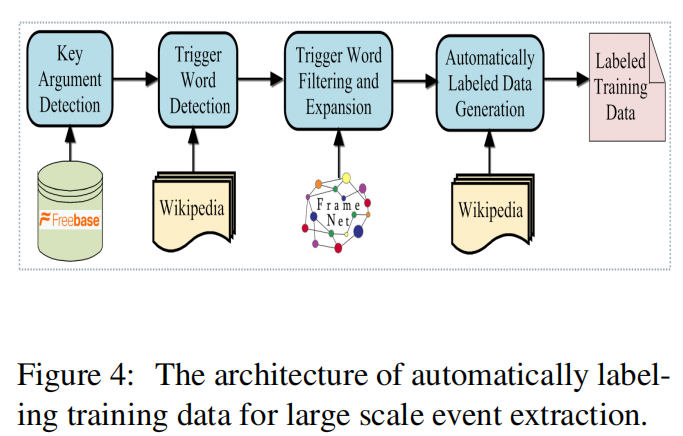
\includegraphics[width = 0.8\textwidth]{2.png}\label{生成数据} \\ %加载图片,缩放至页面的80%
		\caption{生成数据}
		
	\end{figure}
	
	\subsection{Key Argument Detection}
	有些元素在事件中十分的重要,通过这些元素可以轻易地将不同事件区别开来。本文使用Key Rate (KR)来评估一个元素在事件中的重要性。这个重要性取决于两个因素:Role Saliency (角色显著性)和 Event Relevance(事件相关性)。
	\paragraph{Role Saliency (RS):}表示在给定一个特定事件类型下,通过这个元素可以识别出这个事件的程度。也就是,这个元素可以将不同事件区别开的重要程度。RS的定义如下:
	\begin{eqnarray} %%可以自动编号
	{RS\mathop{{}}\nolimits_{{ij}}}=\frac{{Count \left( A\mathop{{}}\nolimits_{{i}},ET\mathop{{}}\nolimits_{{j}} \right) }}{{Count \left( ET\mathop{{}}\nolimits_{{j}} \right) }}
	\end{eqnarray}
	$RS_{ij}$是第j个事件中,第i个元素的重要程度。${Count \left( A\mathop{{}}\nolimits_{{i}},ET\mathop{{}}\nolimits_{{j}} \right) }$是在Freebase中,事件j中,元素i出现的次数。${Count \left( ET\mathop{{}}\nolimits_{{j}} \right) }$是事件j在Freebase出现的次数。
	\paragraph{Event Relevance (ER):}反映这个元素可以将事件抽取出来的能力。如果这个元素出现在每一个事件中,那么这个元素就会有很低的事件相关性。ER的计算式如下:
	\begin{eqnarray}
	{ER\mathop{{}}\nolimits_{{i}}}=log\frac{{Sum \left( ET\mathop{{}}\nolimits_{{}} \right) }}{1+{Count \left( ETC\mathop{{}}\nolimits_{{i}} \right) }}
	\end{eqnarray}
	$ER_{i}$是第i个元素的事件相关性,Sum(ET)是在知识库中所有事件类型的数量。${Count \left( ETC\mathop{{}}\nolimits_{{i}}\right) } $是包含第i个元素的事件类型,最后KR的计算如下:
	\[{{KR\mathop{{}}\nolimits_{{ij}}}=RS_{ij}*ER_{i}}\]
	本文计算了每个事件类型的所有元素,并根据KR进行了排序,然后本文选取了前K个元素作为关键元素。
	
	\subsection{Trigger Word Detection}	
	本节使用上一节的关键元素来标记在维基百科中可能表示事件的句子。本文使用 \textbf{\underline{Standford CoreNLP tool}}来处理维基百科中的原始文本,进行词性标注,命名实体识别。最后,我们选择Freebase中包含事件实例所有关键参数的语句作为表示相应事件的语句。然后我们用这些标记的句子来检测触发词。\\
	
	动词往往会成为表示一个事件的关键。在一个事件类型中,一个动词比其他动词出现的次数多,那么这个动词会触发这个事件。但是,这个动词出现在每一个事件中,就不会触发这个事件。因此我们提出Trigger Candidate Frequency (TCF) 和 Trigger
	Event Type Frequency (TETF)去评估两个方面。最后,使用Trigger Rate (TR)来作为最后这个动词成为触发词的可能性。
	\[{{TR\mathop{{}}\nolimits_{{ij}}}=TCF_{ij}*TETF_{i}}\]
	\[{{TCF\mathop{{}}\nolimits_{{ij}}}=\frac{{Count \left( V\mathop{{}}\nolimits_{{i}},ETS\mathop{{}}\nolimits_{{j}} \right) }}{{Count \left( ETS\mathop{{}}\nolimits_{{j}} \right) }}}\]
	\[{{TETF\mathop{{}}\nolimits_{{i}}}=log\frac{{Sum \left( ET\mathop{{}}\nolimits_{{}} \right) }}{1+{Count \left( ETI\mathop{{}}\nolimits_{{i}} \right) }}}\]
	$TR_{ij}$是在第j个事件类型中,第i个动词的触发概率。${Count \left( V\mathop{{}}\nolimits_{{i}},ETS\mathop{{}}\nolimits_{{j}} \right) }$是第j个事件类型下,包含第i个动词句子的数量。${Count \left( ETS\mathop{{}}\nolimits_{{j}} \right) }$是第j个事件类型的数量。${Count \left( ETI\mathop{{}}\nolimits_{{i}} \right) }$是包含动词i的事件数量。最后,为每个事件选择合适的触发词。
	
	\subsection{Trigger Word Filtering and Expansion}
	通过以上的触发词检测,我们可以得到一个初始的触发词。然而,这个最初的触发词汇是不准确的,并且只包含了动词的触发词,名词触发词被忽略了。本文使用FrameNet来过滤不准确的动词以及扩展名词的触发词。使用词嵌入,将Freebase里面的事件映射到FrameNet的框架里,计算Freebase事件类型与FrameNet中事件框架的语义相似度。公式如下:
	\begin{eqnarray}
	{frame \left.( i \left.) =\mathop{{argmax\text{ }}}\limits_{{j}} \left( similarity \left( e\mathop{{}}\nolimits_{{i}},e\mathop{{}}\nolimits_{{j,k}} \left . \right .\right )\right )\right.\right. }
	\end{eqnarray}
	然后,我们过滤动词,它是在最初的动词触发词词典,而不是在映射框架。我们在映射框架中使用高置信度的名词来扩展触发词汇。

	\subsection{Automatically labeled data generation}
	最后,本文提出Soft Distant Supervision,并用它进行自动生成训练数据。也就是假设任何包含Freebase中所有关键参数和相应触发词的语句都可能以某种方式表示该事件,并且该语句中出现的参数可能在该事件中扮演相应的角色。
	
	\section{Method of Event Extraction}
	在本文中,事件抽取有两个阶段,是一个多分类任务。第一个阶段是\textbf{事件分类},如果在Freebase中,关键元素出现了,那么就进入第二个阶段\textbf{元素识别},进行识别事件中的元素。使用Multi-pooling Convolutional Neural Networks with Multi-instance Learning(DMCNNs-MIL)来进行两个阶段的工作。为了防止错误标签带来的问题,本文在两个DMCNN上使用Multi-instance Learning (MIL)多示例学习。两个DMCNN分别在两个阶段使用多示例学习。在每个包上,目标函数使用交叉熵。
	\[{J \left.(  \theta  \left.) ={\mathop{ \sum }\limits_{{i=1}}^{{T}}{logp \left( y\mathop{{}}\nolimits_{{i}} \left| \mathop{{m}}\nolimits_{{j}}^{{i}}, \theta  \right) \right. }}\right. \right. }\]
	事件j使用最大似然函数,拥有这些元素的情况下,最有可能是哪些事件。
	\[{j\mathop{{}}\nolimits^{{*}}=arg\mathop{{max}}\limits_{{j}}p \left( r \left| m\mathop{{}}\nolimits_{{j}}^{{i}}, \theta  \right) \right. }\]
	采用随机梯度下降法(Adadelta),mini-batches.
	
	\section{Experiments}
	在本节,先人工评估自动标记的数据,然后评估在ACE数据上标记的数据,最后评估DMCNN-MIL在自动标记数据上面的性能。
	\subsection{Our Automatically Labeled Data}
	首先设置超参数,关键元素的个数为2(后面做实验得到的结果),触发词重要程度为0.8。先使用两个关键元素去标记数据,接着使用这些标记数据以及FrameNet来找触发词以及用SDS来生成标记数据。最后生成72611个标记数据。
	\subsection{Manual Evaluations of Labeled Data}
	从自动标记的数据中随机选择500个样本,每个样本由三个人进行标记,自动标记数据的准确率,如表所示。
		\begin{table}[h]
			\centering
			\begin{tabular}{|l|l|}
				\hline
				阶段 & 平均准确率    \\ \hline
				触发词标记 & 88.9    \\ \hline
				元素标记 & 85.4    \\ \hline
			
			\end{tabular}
		
		\end{table}

	\subsection{Automatic Evaluations of Labeled Data}
	本文使用两个方式将自动标记的数据加入到ACE的数据库。
	\begin{enumerate}
		\item 我们删除ACE数据中有这些重复事件类型的人工注释ACE数据,并将自动标记的数据添加到剩余的ACE训练数据中。我们叫扩展数据(ED)。
		\item 我们直接把自动标注的数据加入到ACE相同事件类型中,我们把这个训练数据叫ACE+ED
	\end{enumerate}
	用DMCNN来训练这些数据,并在ACE数据中进行测试。测试结果如下:
		\begin{figure}[h]
			\centering
			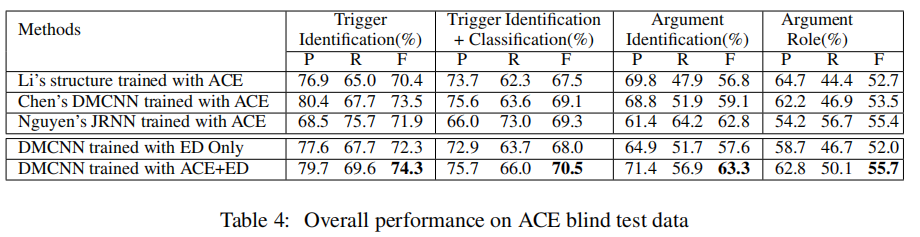
\includegraphics[width = \textwidth]{3.png} \\ %加载图片,缩放至页面的80%
			\caption{测试结果}
		\end{figure}
	这个结果证明自动生成数据是有效的。
	\subsection{Discussion}
	\textbf{Impact of Key Rate}\\
	\begin{table}[h]
	\centering
	\begin{tabular}{|l|l|l|}
		\hline
		特征 & 触发词(F1 )  & 元素(F1)\\ \hline
		ACE & 69.1 & 53.5  \\ \hline
		AEC+RS & 70.1   & 55.3\\ \hline
		AEC+ER & 69.5   & 54.2\\ \hline
		AEC+KR & \textbf{70.5}   & \textbf{55.7}\\ \hline
	\end{tabular}
		
	\end{table}

	\textbf{Impact of Trigger Rate and FrameNet}\\
	在这个部分证明TR和FrameNet找到触发词的有效性。用Grid search来进行寻找最优参数(0.5, 0.6, 0.7, 0.8, 0.9, 1.0)。最后是0.8。
		\begin{figure}[h]
			\centering
			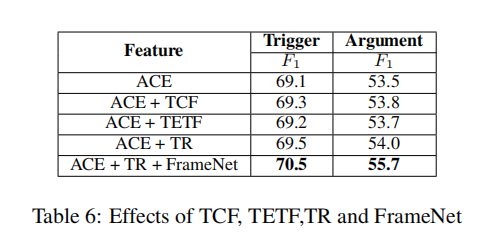
\includegraphics[width = 0.8\textwidth]{4.png} \\ %加载图片,缩放至页面的80%
			\caption{测试结果}
		\end{figure}		
	\subsection{Performance of DMCNN-MIL}
	有两种评估本文方法的方式:held-out and manual evaluation
	\paragraph{Held-out Evaluation}
	用两个标准去评判自动预测事件的准确性:
	\begin{enumerate}
		\item 关键元素和事件类型是否匹配
		\item 事件类型和元素角色是否匹配
	\end{enumerate}
	我们可以看到,多实例学习可以有效地缓解远程监督事件抽取中的噪声问题。
	\begin{figure}[h]
		\centering
		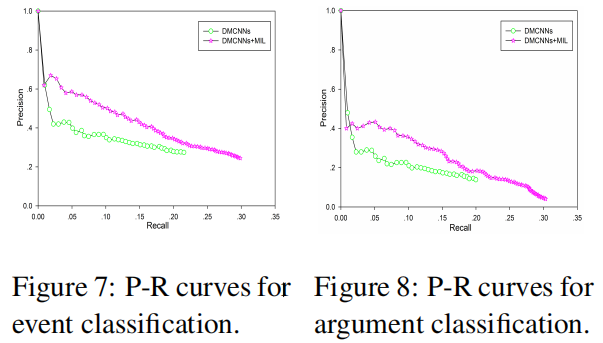
\includegraphics[width = .8\textwidth]{5.png} \\ %加载图片,缩放至页面的80%
		\caption{测试结果}
	\end{figure}
	\paragraph{Human Evaluation}
	这个部分仅仅评估没有在Freebase中出现的事件示例。
	
		\begin{figure}[h]
			\centering
			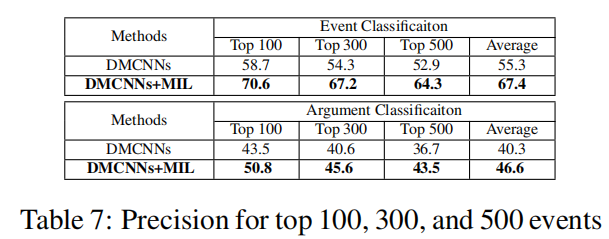
\includegraphics[width = \textwidth]{6.png} \\ %加载图片,缩放至页面的80%
			\caption{测试结果}
		\end{figure}
	可以看出DMCNNs-MIL获得了最好的结果。
	
	\section{Conclusion and Future Work}
	在未来,我们将使用所提出的自动数据标记方法来处理更多的事件类型,并探索使用自动标记的数据来提取事件的更多模型。
\end{document}